\documentclass[10pt,twocolumn,letterpaper]{article}

\usepackage{cvpr}
\usepackage{times}
\usepackage{epsfig}
\usepackage{graphicx}
\usepackage{amsmath}
\usepackage{amssymb}

% Include other packages here, before hyperref.
\usepackage[inline]{enumitem}
\usepackage{multirow}
\usepackage[style=ieee]{biblatex}
\bibliography{../presentation/depth}

% If you comment hyperref and then uncomment it, you should delete
% egpaper.aux before re-running latex.  (Or just hit 'q' on the first latex
% run, let it finish, and you should be clear).
\usepackage[breaklinks=true,bookmarks=true]{hyperref}

\cvprfinalcopy % *** Uncomment this line for the final submission

\def\cvprPaperID{****} % *** Enter the CVPR Paper ID here
\def\httilde{\mbox{\tt\raisebox{-.5ex}{\symbol{126}}}}

% Pages are numbered in submission mode, and unnumbered in camera-ready
%\ifcvprfinal\pagestyle{empty}\fi
\setcounter{page}{1}
\begin{document}

%%%%%%%%% TITLE
\title{Images Classification with Estimated Depth Map
\thanks{This work is our course project for 2016 Spring CS291K Advanced Data Mining, taught by prof. Xifeng Yan in UCSB.}}
\author{Yihui He\thanks{Yihui is a CS 2nd year undergrad, 
from Xi'an Jiaotong University, China. 
Interested in Deep Learning and Computer Vision. 
He is an exchange student at UCSB during 2016 Spring.}\\
Xi'an Jiaotong University\\
%Xi'an, China\\
{\tt\small heyihui@stu.xjtu.edu.cn}
% For a paper whose authors are all at the same institution,
% omit the following lines up until the closing ``}''.
% Additional authors and addresses can be added with ``\and'',
% just like the second author.
% To save space, use either the email address or home page, not both
\and
Metehan Ozten\\
University of California, Santa Barbara\\
%First line of institution2 address\\
{\tt\small m\_ozten@umail.ucsb.edu}
}


\maketitle
%\thispagestyle{empty}

%%%%%%%%% ABSTRACT
\begin{abstract}
We consider the problem of doing image classification using estimated depth 
information. This problem clearly falls into the domain of transfer learning, since we are using a model trained on a set of depth images in order to generate depth maps (additional features) for use in another classification problem using another disjoin set of images. It is a challenging task as no direct depth information is 
provided. Previous related research efforts have been focused on image classification tasks using
RGB images and depth image estimation but none have attempted to use depth image estimations in order to aid image classification over RGB images. Therefore, in this paper we present a way of 
transfering domain knowledge on depth estimation to a seperate image classification task over a disjoint set of training/test data. 
To our knowledge, we are the first to bridge gap between image classification 
and depth estimation.

Specifically, we attempt to implement the recent work by Fayao 
Liu \etal\cite{liu2015deep}, build a RGBD dataset and do image classification 
on the RGBD dataset we built and then compare the performance of both a simple feedforward neural network and a multi-layer convolutional neural network of the RGBD dataset compared to the RGB dataset 
Our project code, models, and example results are available on github: \href{
https://github.com/yihui-he/Depth-estimation-with-neural-network 
}{github.com/yihui-he/Depth-estimation-with-neural-network}
\href{
https://github.com/netzo92/cs291k-FP
}{https://github.com/netzo92/cs291k-FP}
\end{abstract}

%%%%%%%%% BODY TEXT
\section{Introduction}
Estimating depths from a single monocular image depicting 
general scenes is a fundamental problem in computer vision, 
which has found wide applications in scene understanding, 
3D modeling, robotics, etc.
It is a notoriously ill-posed problem, 
as one captured image may correspond to numerous real world scenes\cite{eigen2014depth}. 
it remains a challenging task for computer vision algorithms as no reliable cues can be exploited,
such as temporal information, stereo correspondences, \etc.
Previous work mainly focus on Depth estimation,
using 
geometric\cite{hedau2010thinking,gupta2010estimating,gupta2010blocks} 
or CNN\cite{liu2015deep} approach,
, and Semantic labeling\cite{ladicky2014pulling} with depth information.
Nevertheless, all these works didn't try to do recognition with depth map.

Different from previous efforts, 
we propose to put depth map into practice on classification task.
While extensively studied in semantic labeling and accuracy improvement,
depth map regression has been less explored for classification problems.

Recently, the efficacy and power of the deep
convolutional neural network (CNN) has been discovered and utilized. 
With a CNN, we are able to do depth estimation on a single image\cite{liu2015deep}.
However, most classification tasks still perform on RGB images.
With only RGB images, 
CNN features have been setting new records for a wide variety of vision applications\cite{razavian2014cnn}.
Despite all the successes in depth estimation and image classification,
deep CNN has been less explored for learning on RGBD images, since RGBD datasets are not as widely-used as RGB datasets .
To our knowledge, we are the first to bridge gap between depth estimation and 
image classification.

To sum up, we highlight the main contributions of this work as follows:
\begin{itemize}
\vspace{-.12cm} \item 
We reproduce deep convoluntional neural field on depth estimation problem, 
and get similar results.
\vspace{-.12cm} \item
We create the first RGBD image dataset for CIFAR10.
\vspace{-.12cm} \item 
We define a new metric for ill-posed depth prediction problem.
\vspace{-.12cm} \item 
We prove that depth channel has a better feature representation than R,G,B channels,
and show that training on RGBD images can somehow improve accuracy.
\end{itemize}


%-------------------------------------------------------------------------
\section{Related Work}
Convolutional networks have been applied with great success for object 
classification and detection. ConvNets have recently been applied to a variety 
of other tasks, like depth estimation. Depth estimation from single image is 
well addressed by Liu\etal\cite{liu2015deep} and Eigen\etal 
\cite{eigen2015predicting}. They both agree that depth estimation 
is an ill posed problem, since there's no real groud truth depth map. By 
contrast, we define transfer learning accuracy metric for depth estimation 
model. It becomes easier to compare performance of different depth estimation 
model.

Depth map has been successfully applied to some problems. based on depth 
information, performance improvement on semantic 
labeling\cite{eigen2015predicting} has been seen. however, depth map hasn't 
been combined with classification task. to our knowledge, we are the first to 
bridge gap between depth estimation and image classification.

our work builds upon state-of-the-art depth estimation model\cite{liu2015deep}
which is a two loss neural network. we build rgbd dataset, and investigate 
quality and potential usage of depth map intensely. moreover, we improve 
accuracy of image classification task with depth map.

%-------------------------------------------------------------------------
\section{Deep Convolutional Neural Field}
We present the details of deep convolutional neural field model we used for 
depth estimation in this section. 
\subsection{Theory and Architecture}
The goal here is to infer the depth of each pixel in a single image depicting 
general scenes. we make the common assumption that an image is composed of small 
homogeneous regions (superpixels). 
Let $x$ be an image and $y=[y_1,...,y_n]^T\in R^n$ be a vector of continuous 
depth values corresponding to all n superpixels in x. We model the conditional 
probability as softmax:
\begin{equation}
Pr(y|x)=\frac{exp(-E(y,x))}{\sum_i 
exp(E(y_i,x))}
\end{equation}
where $E$ is energy function.
To predict the depths of a new image, we solve the maximum a posteriori (MAP) 
inference problem: 
\begin{equation}
 \label{eq:inference}
y^{\star}=\arg\max\limits_y Pr(y|x). 
\end{equation}
We formulate the energy function as a 
typical combination of unary potentials U and pairwise potentials V over the 
nodes (superpixels) N and edges S of the image x:
\begin{equation}\label{eq:energy}
E(y, x) = \sum_{p \in {\cal N} } U(y_{p}, x) 
	 + \sum_{(p,q) \in {\cal S}} V(y_{p}, y_{q}, x).
\end{equation}
The unary term U aims to regress the depth value from a single superpixel. The 
pairwise term V encourages neighbouring superpixels with similar appearances 
to take similar depths. We aim to jointly learn U and V in a unified CNN 
framework.
In Figure.\ref{fig:arch} , we show a sketch of our deep convolutional
neural field model for depth estimation. As we can see, the whole network is 
composed of a unary part, a pairwise part and a CRF loss layer.
\begin{figure}
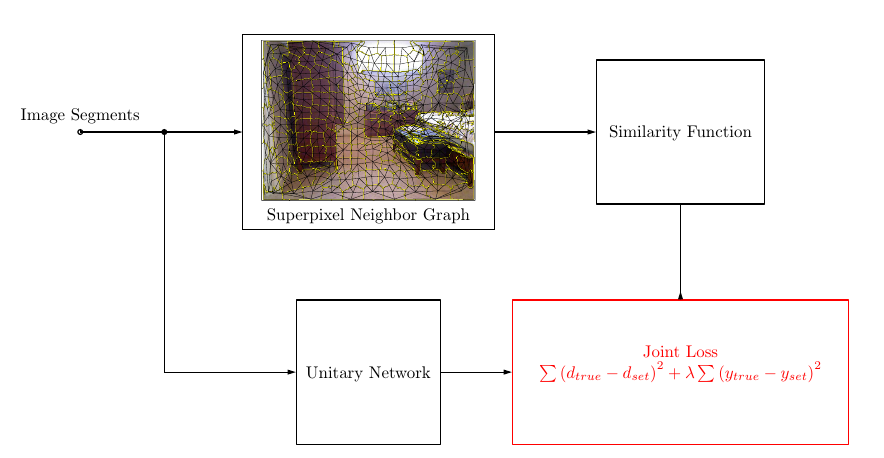
\includegraphics[width=.9\linewidth]{../presentation/arch.png}
\caption{Deep Convolutional Neural Field model}
\label{fig:arch}
\end{figure}

For an input image, which has been segmented into n superpixels, we 
consider image patches centred around each superpxiel centroid. The unary part 
then takes all the image patches as input and feed each of them to a CNN and 
output an n-dimentional vector con- taining regressed depth values of the n 
superpixels. The network for the unary part is composed of 5 convolutional and 
4 fully-connected layers with details in Figure.\ref{fig:unary}. 
\begin{figure*}
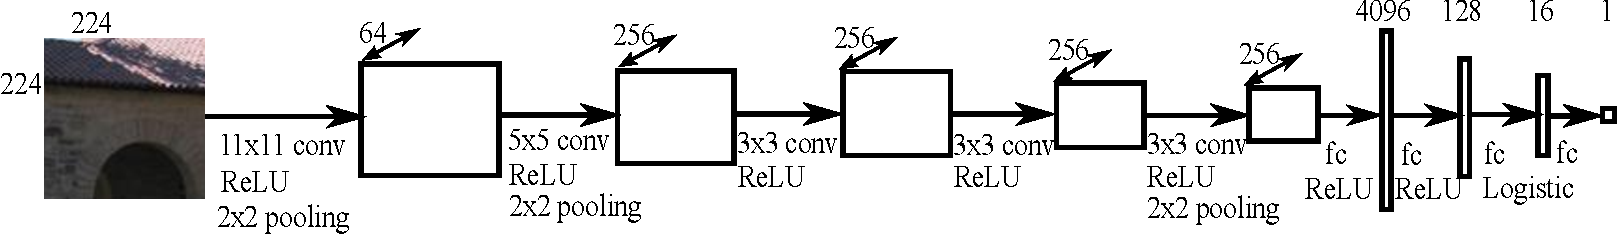
\includegraphics[width=\linewidth]{../presentation/fig/cnn_unary.pdf}
\caption{unary part of Deep Convolutional Neural Field model}
\label{fig:unary}
\end{figure*}

Kindly note that the CNN parameters are shared across all the su- perpixels. 
The pairwise part takes similarity vectors (each with K components) of all 
neighbouring superpixel pairs as input and feed each of them to a 
fully-connected layer (parameters are shared among different pairs), then output 
a vector containing all the 1-dimentional similarities for each of the 
neighbouring superpixel pair. The CRF loss layer takes as input the outputs from 
the unary and the pairwise parts to minimize the negative log-likelihood.
\subsubsection{Unary part}
The unary potential is constructed from the output of a CNN by considering the 
least square loss:
\begin{equation}\label{eq:unary}
U(y_{p}, x;\theta) = (y_p - \hat{y}_p (\theta))^2, \;\; \forall p=1,...,n.
\end{equation}
Here $\hat{y}_p$ is the regressed depth of the superpixel $p$ parametrized by 
the CNN parameters $\theta$. The network architecture for the unary part is 
depicted in Figure.\ref{fig:unary}. It is composed of 5 convolutional layers 
and 4 fully connected layers. The input image is first segmented into 
superpixels, then for each superpixel, we consider the image patch centred 
around its centroid. Each of the image patches is resized to 224×224 pixels and 
then fed to the convolutional neural network. Note that the con- volutional and 
the fully-connected layers are shared across all the image patches of different 
superpixels.
\subsubsection{Pairwise part}
We construct the pairwise potential from 3 types of similarity observations: 
color difference, color histogram difference and texture 
disparity\cite{ojala1994performance}. Each of them enforces smoothness by 
exploiting consistency information of neighbouring superpixels:
\begin{equation}
 \label{eq:pairwise}
V(y_{p}, y_{q}, x; \beta) = \sum_{k=1}^K \beta_k S_{pq}^{(k)}(y_p - y_q)^2, 
\;\forall p,q=1,...,n.
\end{equation}
Here, $K=3$ in our case. $S_{pq}$is similarity of two neighour superpixels $p$ 
and $q$. $\beta$ is trainable parameters, so we can let CNN decide which 
similarity is more improtant. 

\subsection{Implementation Details}
We implement the network training on Make3D\cite{saxena2005learning} dataset 
with Tensorflow\cite{tensorflow2015-whitepaper}. Make3D dataset contains 
more outdoor scenes, which makes it easier for us to transer learning on 
CIFAR10 dataset in the following section. During each SGD iteration, 
around ∼ 700 superpixel image patches t need to be processed. Different from 
orginal implementation\cite{liu2015deep}, Since we have enough memory, we feed 
700 superpixel image patches into memory at once. Other parts of implementation 
are similar.

During implementation, we initialize the first 6 layers of the unary part in 
Figure.\ref{fig:unary} using a CNN model trained on the ImageNet 
from\cite{chatfield2014return}. First, we do not back propa- gate through the 
previous 6 layers by keeping them fixed and train the rest of the network
with momentum 0.9, learning rate 0.0001, and weight decay 
0.0005. Then we train the whole network with the same momentum and weight decay.

\subsection{Experiment}
We measure our performance on Make3D dataset and compare our result with Liu 
\etal \cite{liu2015deep} as a sanity check. 

The Make3D dataset contains 534 images depicting outdoor scenes. As pointed out 
in \cite{liu2014discrete}, this dataset is with limitations: the maximum value 
of depths is 81m with far objects are all mapped to the one distance of 81 
me- ters. As a remedy, two criteria are used to report the prediction error (C1) 
Errors are calculated only in the re- gions with the ground-truth depth less 
than 70 meters; (C2) Errors are calculated over the entire image. We follow this 
protocol.
Performance is shown in Table\ref{tab:sanity}. 
You can see that
our model achieve pretty close result, which allows us do further research on depth map.
\begin{table} \center
\resizebox{\linewidth}{!} {
\begin{tabular}{ | l |  c  c  c | c  c  c |}
\hline 
\multirow{3}{*}{{{Method}}} &\multicolumn{3}{c|}{Error(C1)} 
&\multicolumn{3}{c|}{Error(C2)} \\
&\multicolumn{3}{c|}{(lower is better)} &\multicolumn{3}{c|}{(lower is better)} 
\\
\cline{2-7}
&rel &log10 &rms &rel &log10 &rms  \\
\hline
%
%
Our implementation &0.335&0.137&9.49&0.338&0.134&14.60 \\
Original paper    &\textbf{0.314}&\textbf{0.119}  &\textbf{8.60}  
&\textbf{0.307} 	 &\textbf{0.125}	 &\textbf{12.89} \\
\hline
\end{tabular}
}
\caption{Sanity check (\textbf{Bold} is better)}
\label{tab:sanity}
\end{table}

In Figure\ref{fig:depthest} we also show depth maps our model learned.
\begin{figure}
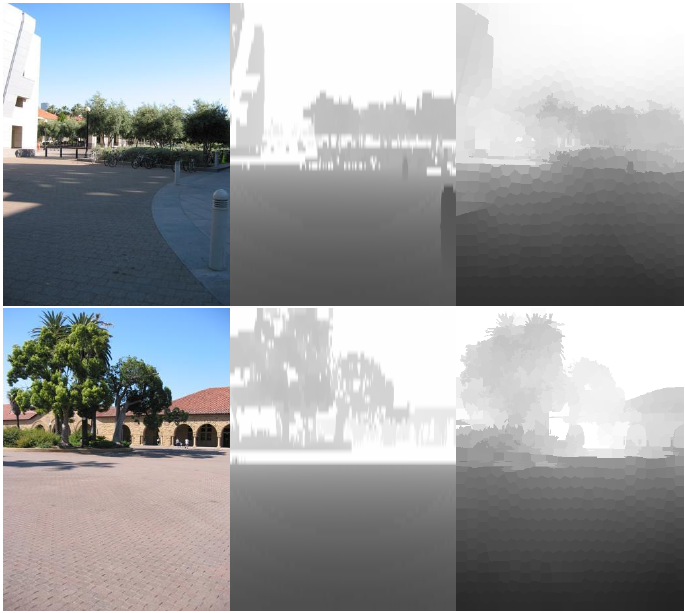
\includegraphics[width=\linewidth]{../learntd.png}
\caption{original image, ground truth, depth estimation(from left to right)}
\label{fig:depthest}
\end{figure}

%-------------------------------------------------------------------------
\section{RGBD Image for Classification}
Recent depth image research works
mainly focus on depth estimation\cite{liu2015deep} 
and segementation with depth image\cite{eigen2015predicting}.
And we\rq{}ve witnessed significant improvement on depth estimation accuracy in these years. 
However, most image classification tasks nowadays are still performed on RGB images.
So we want to transfer depth knowledge learned by depth estimation model to image classification tasks.
In this section, 
we first build a RGBD imageset for CIFAR10\cite{krizhevsky2009learning}, 
based on trained deep convolutional neural field model in the previous section. 
To investigate the effect of depth channel on image classification task, 
we design two experiments. 
Finally, we propose a new metric for depth estimation performance measurement.

\subsection{Build RGBD CIFAR10 Dataset}
Since the Deep Convoluntional Neural Field model accepts images that are 
much larger that CIFAR10 tiny images(32x32), we build RGBD dataset as follow:
\begin{enumerate}
\item resize CIFAR10 tiny image(32x32x3) to normal size(400x400x3) in order to 
feed in CNF.
\item perform depth estimation on normal size image.
\item resize the output image(depth image, 400x400x1) back to tiny 
image(32x32x1).
\item combine RGB and D channels together as our RGBD image(32x32x4).
\end{enumerate}
Figure\ref{fig:dataset} shows the transer learning procedure.
\begin{figure}
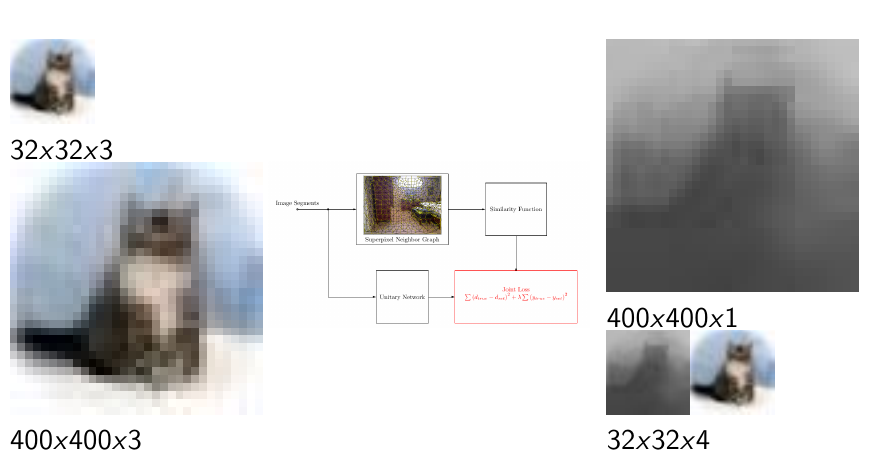
\includegraphics[width=\linewidth]{../dataset.png}
\caption{Transer Learning: Build RGBD CIFAR10 dataset}
\label{fig:dataset}
\end{figure}
Since there is no ground truth depth image for CIFAR10 dataset, we can\rq{}t directly 
know whether depth estimation for these tiny images is successful or not. 
However, we can infer this undirectly in two ways. 
On the one hand, we can look at these depth images
and make sure that most of them is reasonable.
Figure\ref{fig:tiny} shows some depth maps.
On the other hand, we use the accuracy results of two experiments as a new metric to 
compare different depth map quality.
\begin{figure}
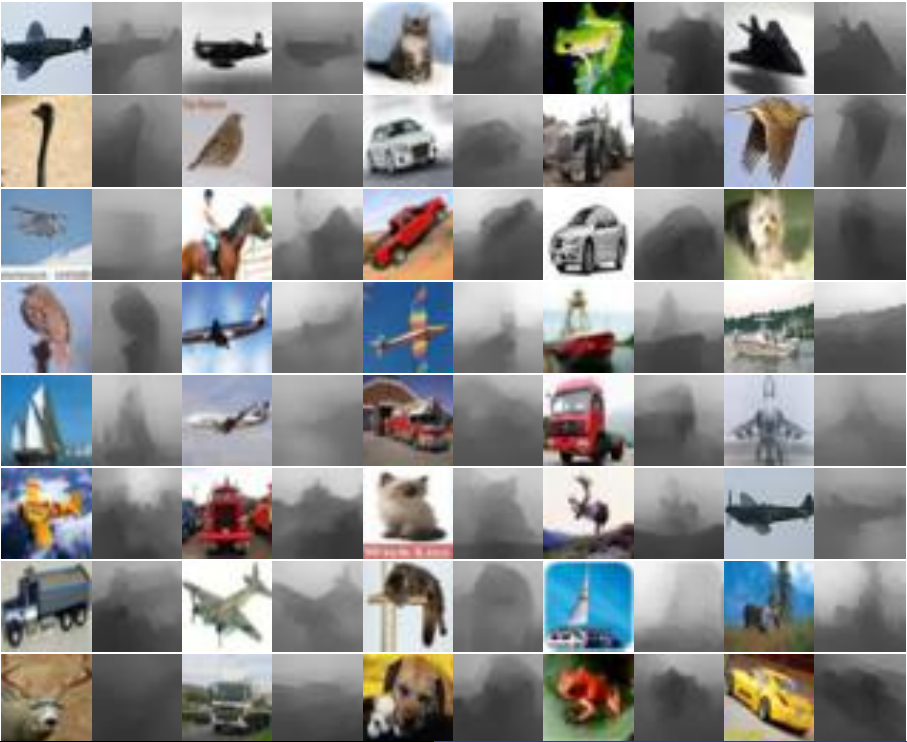
\includegraphics[width=\linewidth]{../tiny.png}
\caption{Depth map estimated by deep convoluntional neural field}
\label{fig:tiny}
\end{figure}

\subsection{Classification Task on RGBD CIFAR10}
In order to make it easier to show effect of depth channel,
 we employ a simple two layer neural network for classification task.
 The architecure for learning on RGBD dataset is shown in Figure\ref{fig:tarch}. 
 \begin{figure}
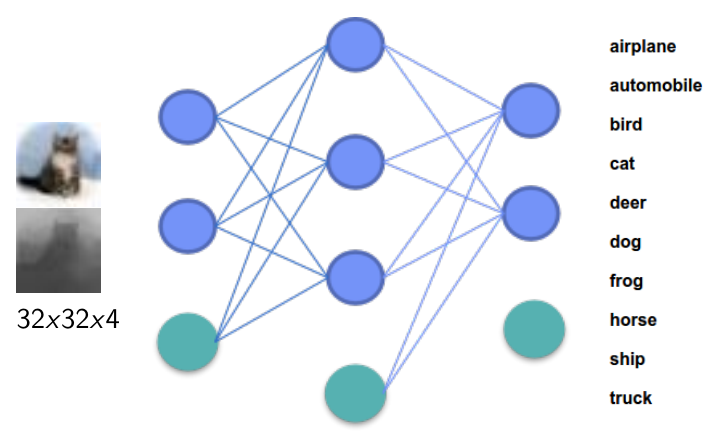
\includegraphics[width=\linewidth]{../Tarch.png}
\caption{Learning on RGBD dataset}
\label{fig:tarch}
\end{figure}
The number of neurons in the input layer depends on input.
If input is a single channel(R,G,B,D), we have 32x32 neurons.
The amount of hidden neurons is not determined. We perform fine tuning 
for each situation. The number of output neurons is always number of classes(10 classes
for CIFAR10). Technical details of our architecture is shown in Table\ref{tab:details}. 
Hyperparameters not dicussed here will be fine tuned.
\begin{table}
\begin{center}
\begin{tabular}{|l|l|l|l|}
\hline
regularization&Activation&Update&batch\\
\hline
Dropout&ReLU&Momentum&128\\
\hline
\end{tabular}
\end{center}
\caption{Archtecture details for classification task on our new RGBD dataset}
\label{tab:details}
\end{table}


\subsection{Experiment}
We measure depth map quality in two ways. 
First, we train neural network on R, G, B, D channel as input respectively.
And compare their loss and accuracy. 
Second, we train neural network on RGB, RGBD respectively. 
And compare their loss and accuracy.

\subsubsection{R vs G vs B vs D}
We perform fine tuning on each channel. So that their performances are approximately optimal.
Figure\ref{fig:channeltrain} shows training accuracy comparision through time. 
Figure\ref{fig:channeltest} shows validation accuracy comparision through time. 
\begin{figure}
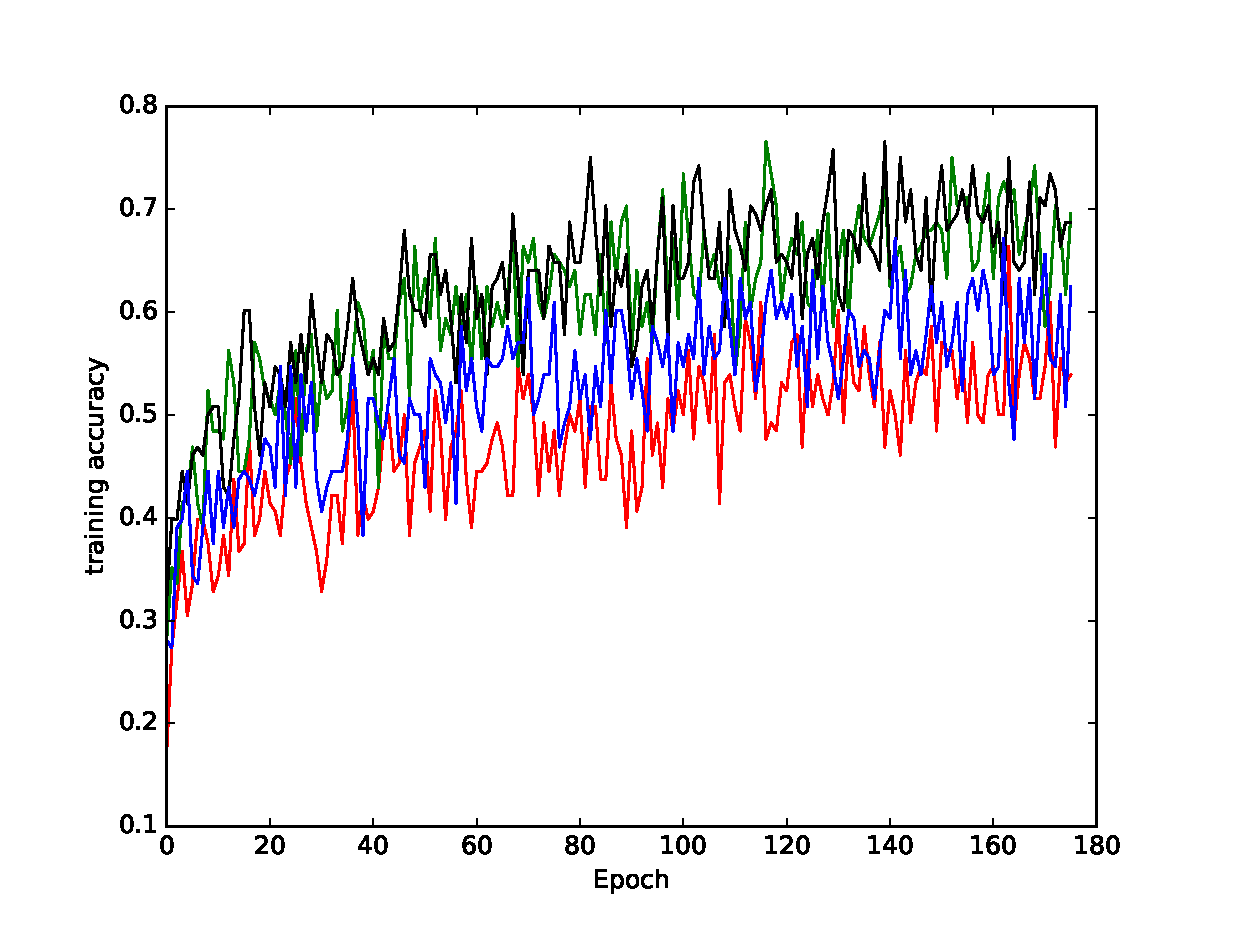
\includegraphics[width=\linewidth]{../presentation/train.eps}
\caption{R vs G vs B vs D, training time}
\label{fig:channeltrain}
\end{figure}
\begin{figure}
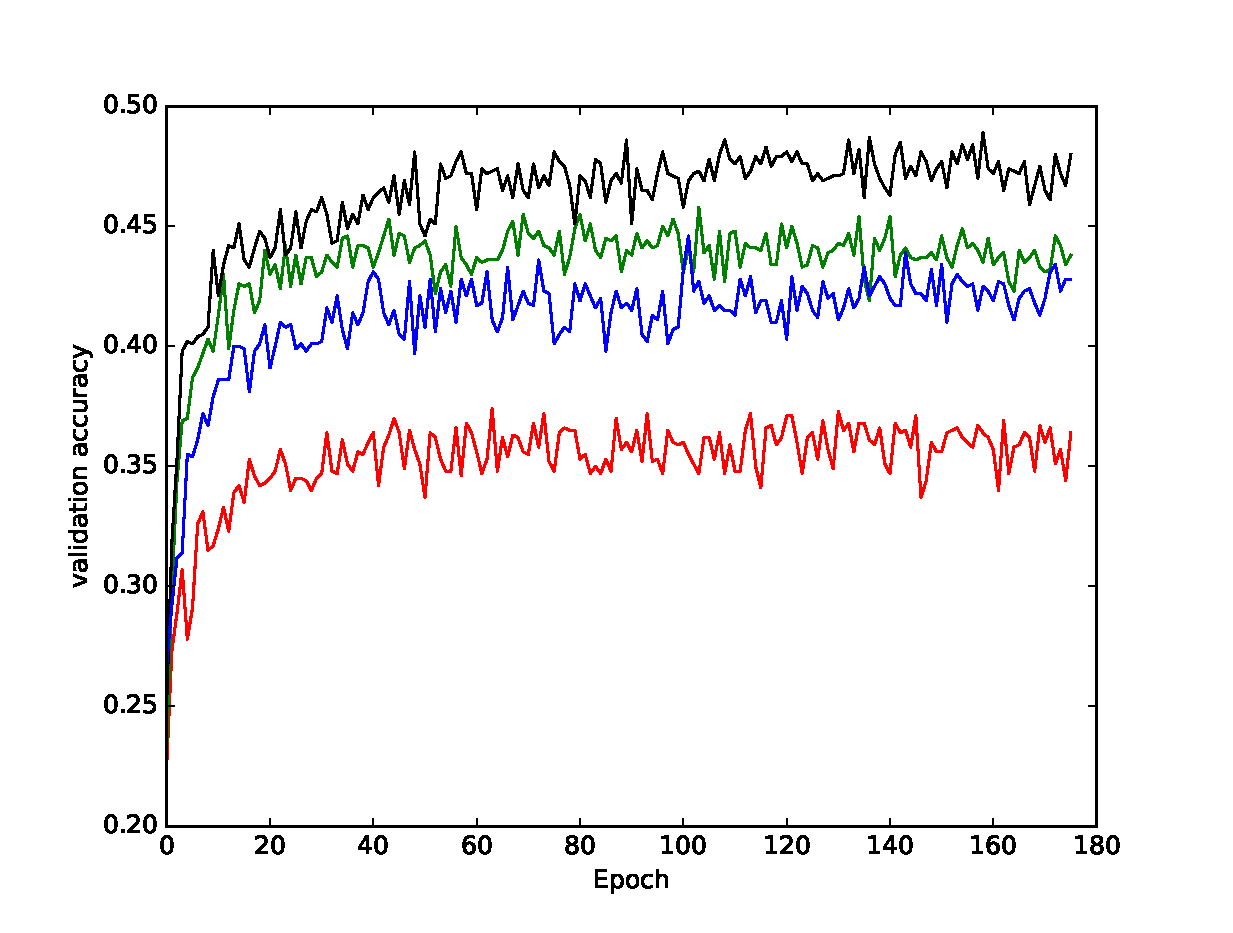
\includegraphics[width=\linewidth]{../presentation/test.eps}
\caption{R vs G vs B vs D, testing time}
\label{fig:channeltest}
\end{figure}

You can see that, at testing time, depth channel out perform R,G,B channels 
under the same architecture.
It implies that, depth channel has a better feature representation than R, G, B channels.

\subsubsection{RGB vs RGBD}
We perform fine tuning for both RGB and RGBD situations.
 So that their performances are approximately optimal.
Figure\ref{fig:mixtrain} shows training accuracy comparision through time. 
Figure\ref{fig:mixtest} shows validation accuracy comparision through time. 
\begin{figure}
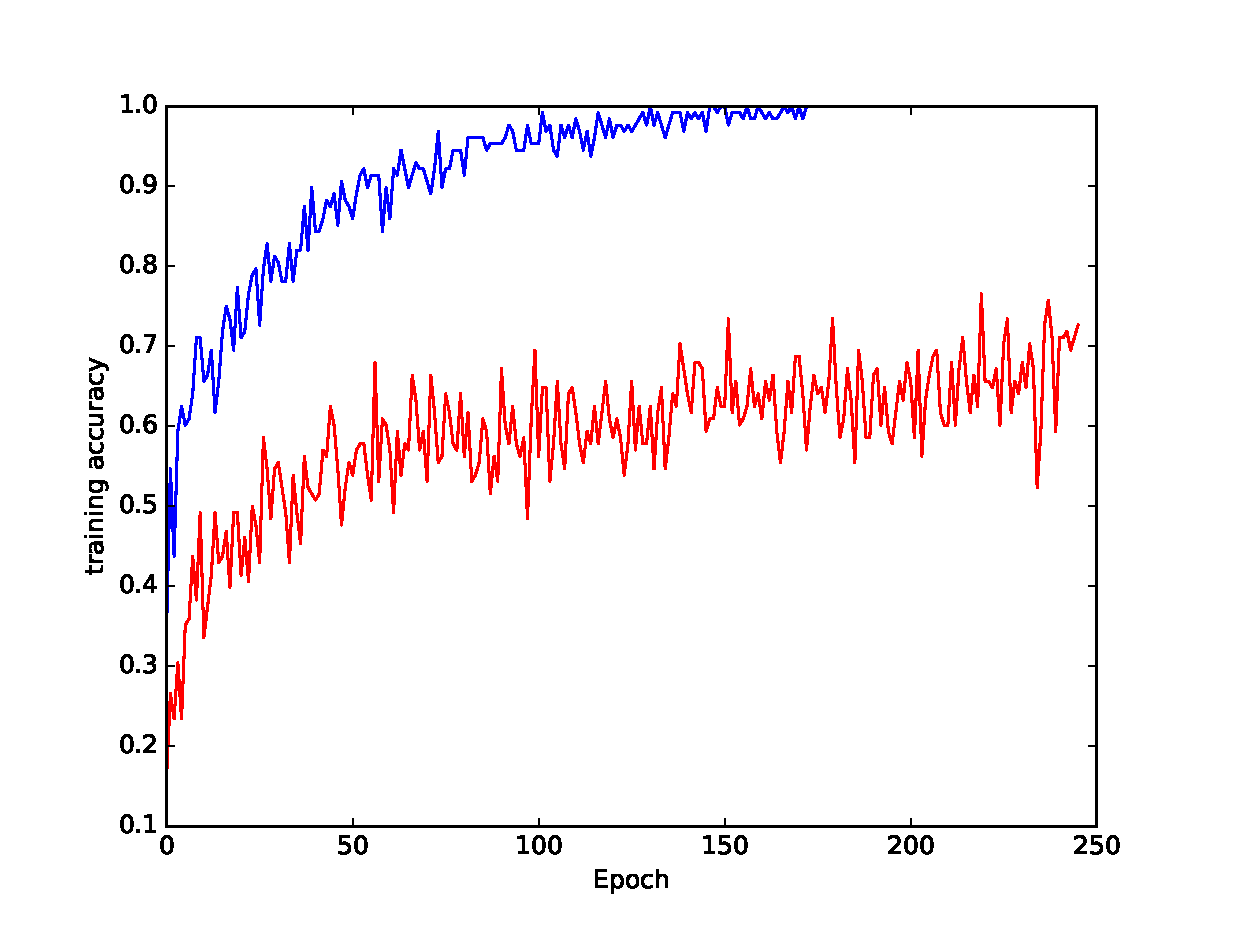
\includegraphics[width=\linewidth]{../presentation/together_train.eps}
\caption{RGB vs RGBD, training time(RGBD:blue, RGB:red)}
\label{fig:mixtrain}
\end{figure}
\begin{figure}
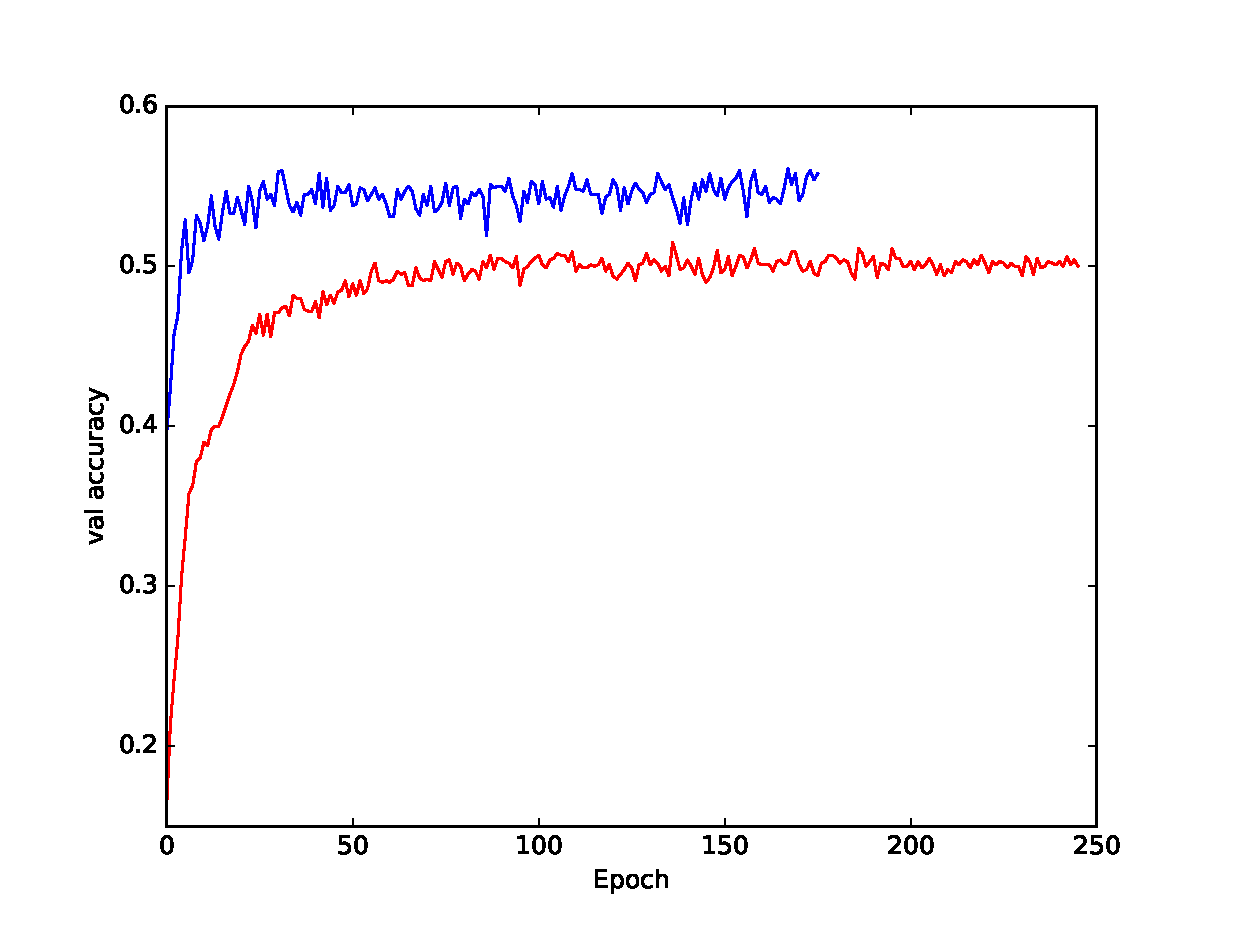
\includegraphics[width=\linewidth]{../presentation/together_test.eps}
\caption{RGB vs RGBD, testing time(RGBD:blue, RGB:red)}
\label{fig:mixtest}
\end{figure}

We get {\bf56\%} and 52\% validation accuracy with RGBD and RGB dataset respectively.
This can be seen as a sign that depth map brings extra knowledge
 learned by deep convoluntional neural field to our classification task.

You can also notice that, although RGBD dataset have more inputs and neurons,
  it has a much higher converge rate than RGB dataset. 
 It can be interpreted as a better feature representation brought by depth map.



%-------------------------------------------------------------------------
\section{Further Work}
\subsection{Depth Estimation}
We\rq{}ve mentioned that depth estimation is an ill-posed problem, 
since we can not find the really ground truth depth map to compare performance of 
different depth estimation models.
However, using the accuracy metric we proposed, performance can be measured 
undirectly.
The only drawback is that our running on our metric need much more time than other metrics.
If we have more time, we\rq{}ll measure performance of existing depth estimation models
 and give a summary.
 
 
\subsection{Learning on RGBD Dataset}
In our experiment, we didn\rq{}t 
employ state-of-the-art image classification model\cite{he2015deep} for simplicity.
We consider to test RGBD dataset on that model. 
Maybe we can witness accuracy surpassing current record.

We also plan to build more RGBD dataset and publish them for research usage.

\subsection{Learning on RGBD(ground-truth) vs RGBD(estimated)}
Compare the accuracy of Learning on RGBD(ground-truth) vs RGBD(estimated).

%-------------------------------------------------------------------------
\section{Conclusion}
We successfully reproduce the state-of-the-art depth estimation model.
We create the first RGBD image dataset for CIFAR10, and investigate its quality 
using our metric.
We define a transfer learning accuracy metric for depth prediction problem.
On RGBD CIFAR, we prove that depth channel has a better feature representation.
We also show that training on RGBD images can somehow improve image 
classification accuracy.


\section*{Role Clarification}
We divide our teamwork as follow. {\bf Yihui}'s contribution:
\begin{enumerate*}
\item proposes idea. 
\item implement deep convolutional neural field. 
\item create RGBD CIFAR10 dataset. 
\item do experiment for 2-layer neural network on RGBD dataset.
\item prepare presentation.
\item edit final report.
\end{enumerate*}
{\bf Metehan}'s contribution:
\begin{enumerate*}
\item discuss idea.
\item implement and do experiment for AlexNet on RGBD dataset. 
\item prepare presentation. 
\item edit final report.
\end{enumerate*}

{\small
\printbibliography
}

\end{document}
